\subsection{Jet Transverse Momentum Shift}

The asymmetries calculated using the 2006 RHIC data are plotted against the
ratio of the charged pion \(p_{T}\) and the ``true'' \(p_{T}\) of the away-side
jet, which incorporates a number of corrections to the actual measured jet
\(p_T\). Various factors bias this measured quantity, including pileup tracks in
the TPC, finite resolution effects, possible detector miscalibrations,
out-of-cone hadronization of fragmenting partons, and in-cone underlying event
effects. The pileup and finite energy resolution are detector effects which can
be corrected in the analysis, while the remaining sources of bias are best
accounted for using a systematic uncertainty.

\subsubsection{Jet $p_T$ Scale Corrections}

TPC pileup has a relatively small effect on the jet momentum in the 2006 run. An
event-mixing analysis using zerobias data concluded that pileup adds an average
of 50 MeV to each jet. The bin migration caused by the $\sim$ 25\% jet energy
resolution results in a much larger \(p_T\) bias. This effect is investigated by
running the jet reconstruction algorithm on final-state particles in the Pythia
record to generate a ``particle'' jet and comparing the \(p_{T}\) of that jet
with the \(p_{T}\) of the ``detector'' jet formed from the tracks and towers of
the full detector simulation. The comparison is repeated for a broad envelope of
calibration parameters, tracking efficiencies, and detector states in order to
account for a possible detector miscalibration.

The hadronization and underlying event biases are not accounted for in the above
analysis. Out-of-cone hadronization is subprocess-dependent, since quark jets
typically have a harder fragmentation profile than gluon jets, while the
underlying event effect is isotropic in \(\eta \times \phi\) space and largely
independent of jet \(p_T\). The two effects are closely connected in the Pythia
Monte Carlo simulations. The combined effect from these two sources of bias was
estimated by comparing jets at the ``fragmented parton'' level with the particle
jets described above. In simulations of fragmented parton jets the underlying
event and hadronization processes are turned off.

Figure~\ref{fig:jet-pt-shift} plots the size of the shift from detector jet
\(p_T\) to particle jet \(p_T\) in bins of detector \(p_T\). The error bars
represent statistical uncertainties on the size of the shift, while the square
brackets denote combined systematic uncertainties from the detector
miscalibration envelope and the hadronization and underlying event effects. The
solid line is a polynomial fit to the data points:
%
\begin{equation}
  \Delta p_T = 1.538 - 0.1561*p_T - 0.001691*p_T^2.
\end{equation}
%
This shift is applied to each accepted jet before calculating the fragmentation
variable ``z'' used in the 2006 asymmetry analysis.

\begin{figure}
  \centering
  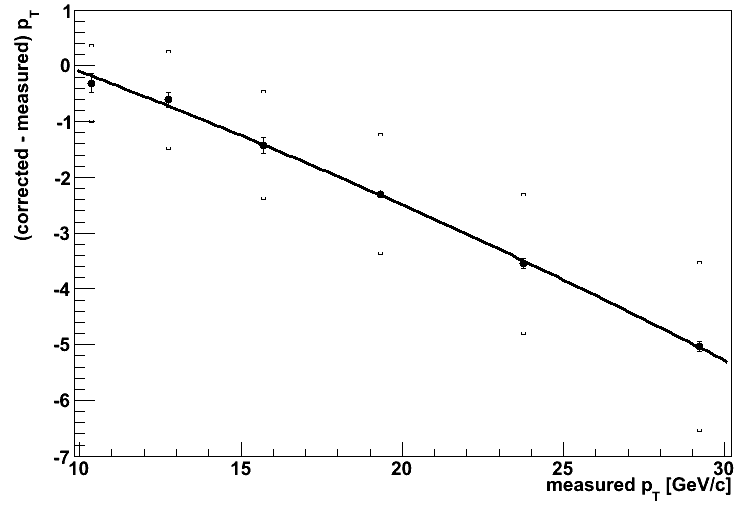
\includegraphics[width=0.7\textwidth]{figures/jet-pt-shift}
  \caption{Correction to measured jet $p_T$.  The data points represent the size of the shift in each measured jet $p_T$ bin, with statistical uncertainties attached.  The solid line is a polynomial fit to those data points, and the outer error bars represent systematic uncertainties due to detector miscalibration, out-of-cone hadronization, and underlying event effects summed in quadrature.}
  \label{fig:jet-pt-shift}
\end{figure}

\subsubsection{Effect on $A_{LL}$}

The bias on \(A_{LL}\) introduced by a systematic error in the jet \(p_T\) scale
corrections is estimated by a maximum extent uncertainty. We evaluate \(A_{LL}\)
using new \(p_T\) shift parameterizations generated from fits to the 1 $\sigma$
total uncertainty bands on the nominal \(p_T\) shift. The average magnitude of
the change in \(A_{LL}\) obtained using these alternative \(p_T\) shifts gives
us the size of the systematic uncertainty. The final values for this uncertainty
are given in Table~\ref{tab:syst-pt-shift}.

\begin{table}
  \centering
  \begin{tabular}{|c||c|c||c|c|}
    \hline
    $z$ & $\pi^-~\delta A_{LL}$ & $\pi^+~\delta A_{LL}$ \\
    % \multirow{2}{*}{$z$} & \multicolumn{2}{c}{$\delta A_{LL}$ ($10^{-2}$)} \\
    % \cline{2-3}
    % & $\pi^-$ & $\pi^+$ \\
    \hline
    0.20 - 0.30 & 0.003 &  0.004 \\
    0.30 - 0.45 & 0.005 &  0.007 \\
    0.45 - 0.65 & 0.016 &  0.016 \\
    0.65 - 1.00 & 0.010 &  0.016 \\
    \hline
  \end{tabular}
  \caption{Systematic uncertainty on $A_{LL}$ due to possible errors in the correction from detector jet $p_T$ to true jet $p_T$.}
  \label{tab:syst-pt-shift}
\end{table}
